\documentclass[12pt,titlepage]{article}
\usepackage{multicol}
\usepackage{fullpage}
\usepackage{graphicx}
\title{I need a title\\\small{Version 0.1}}
\author{Matthew Caron}

\begin{document}
\maketitle
\begin{multicols}{2}

  \tableofcontents
  \newpage

  \section{Introduction}

  I wrote these rules because of my general dissatisfaction with
  microarmor rules currently on the market. Over the past ten years, I
  have spent hundreds of dollars on dozens of rule sets, and examined
  even more free ones. I found all of them to one of: not cover the
  time periods I wanted, be too complex, or not be generic enough to
  cover miniatures by various manufacturers. This rule set is a direct
  response to these issues. They aim to be simple, clear, and
  reasonably realistic.

  \subsection{Design Principles}

  \begin{enumerate}
  \item Game play should be simple, allowing for a fast pace of
    game. A reasonably-sided game consisting of a half-dozen
    squadrons of vehicles and units of infantry should take less
    than an hour to play.
  \item To futher the above, this means as much math as possible
    should be front-loaded as part of the unit creation process.
  \item To further the first item, multiple attacks should be able
    to be rolled as a group, to make them go more quickly.
  \item Troop quality matters as much as, if not more, than
    equipment. Better troops are more effective in combat, are more
    mobile, less likely to rout, etc.
  \item Play should alternate with each player taking turns moving
    units, in order to keep both players actively engaged in the
    game, rather than one player doing nothing as the other player
    moves all his units.
  \item Turns should be of variable length. This models a variety
    of things - fog of war, interrupting people's movement,
    etc. Make it a function of the troop quality, and it models that
    too.
  \end{enumerate}

  \subsection{Meta-Rules}
  \begin{enumerate}
  \item {\bf Don't be a tool} - This is a game. Games are supposed to
    be fun. If you come to a disagreement, go with what logically
    makes sense dealing with reality - don't be a rules-lawyer arguing
    semantics of language. These rules are written to be clear and
    plain, but not all-encompassing.
  \item You can always premeasure anything.
  \item These are miniatures. They can't hide behind things nicely. If
    you state that you are trying to do something (as in ``these guys
    are cowering behind this wall, not trying to shoot you''), then
    they are (and, since they haven't shot you, you haven't shot them,
    it's all fair).
  \item All die rolls use 6 sided dice. In this document ``die'',
    ``dice'' and ``d6'' all refer to dice with 6 sides.
  \item A die roll of 1 always fails, 6 always succeeds.
  \end{enumerate}

  \end{multicols}

  \section{The unit card}
  
  A couple of example unit cards are shown below:

  \begin{center}
    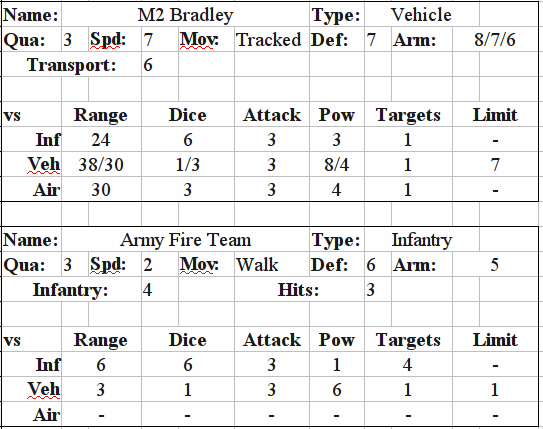
\includegraphics[scale=0.75]{cards.png}
  \end{center}

  \begin{multicols}{2}

    Each card has the following fields:

    \begin{description}
    \item General fields:
      \begin{description}
        \item{\bf Name} - The name of the unit
        \item{\bf Type} - The type of the unit - either {\bf Inf}
          (Infantry), {\bf Veh} (Vehicle), or {\bf Air} (Aircraft).
        \item {\bf Qua} (Quality) - zThe quality of the unit - from 1
          to 5.
        \item {\bf Spd} (Speed) - The movement speed of the unit, in
          inches.
        \item {\bf Mov} (Movement type) - The type of movement the
          unit uses.
        \item {\bf Def} (Defense) - The unit's defense value - the
          attacker compares his attack roll plus the attack value of the
          weapon and must roll greater than or equal to the defense
          number.
        \item {\bf Arm} (Armor) - The armor value of the unit - the
          attacker compares his penetration roll plus the power value
          of the weapon and must roll greater than or equal to the armor
          number. Note that some units have several numbers separated by
          slashes. This notation is either front/side/rear or
          front/rear, depending on the unit type.
      \end{description}
    \item Weapon system fields:
      \begin{description}
      \item {\bf vs} - The type of unit which the weapon system can be
        used to attack. One of {\bf Inf} (Infantry) {\bf Veh}
        (Vehicle) or {\bf Air} (Aircraft).
      \item {\bf Range} - The range of the weapon system for the given
        target type.
      \item {\bf Dice} - The number of dice the attacker gets to roll
        when attacking with the given weapon system (barring any
        damage to the unit), see {\bf Hits} below. 
      \item {\bf Attack} - The attack value of the weapon system. The
        attacker rolls his attack dice and adds this value to each of
        them, comparing the result to the defender's {\bf Def}
        value. Every number which is greater than or equal to the {\bf
          Def} is a hit. 
      \item {\bf Pow} - The power of the weapon system. The attacker
        rolls a die for each hit and adds this value to each of them,
        comparing the result to the defender's {\bf Arm} value. Every
        number which is greater than or equal to the {\bf Arm} is a
        penetrating hit, and incurs a hit. 
      \item {\bf Targets} - The attacker may split the attack dice
        amongst this many targets.
      \item {\bf Limit} - The weapon system can make this many attacks
        during the course of the game.
      \end{description}
      
    \item Notes on the weapon system fields:
      \begin{itemize}
      \item For {\bf vs}, {\bf Range}, {\bf Dice}, {\bf Attack}, {\bf
        Pow} and {\bf Targets}, a ``-'' means that the unit has no
        weapon system which can be used against that unit type. For
        {\bf Limit}, it means that there is no limit to the number of
        attacks which can be made wih the weapon system.
      \item Two numbers separated by a slash indicate primary and
        secondary attacks. Typically, this is because the vehicle has
        a long and short range weapon system, or a powerful attack
        with limited ammunition, and a weaker attack with much more
        ammunition. You make elect to make an attack with either
        weapon system which is in range. Note that not all fields may
        have the primary/secondary notation. If so, then both weapon
        systems use the same value.
      \end{itemize}
    \end{description}

    In addition, some cards have the following fields:
    \begin{description}
      \item {\bf Transport} - The number of points of infantry the
        unit can transport.
      \item {\bf Infantry} - The unit is infantry, and takes up this
        many points of space in a {\bf Transport}.
      \item {\bf Hits} - The unit can incur this many hits before it
        is no longer combat effective and is removed from the
        table. Each hit reduces the number of dice rolled on an attack
        by 1. If this reduces the number of dice to 0, an attack
        cannot be made against that target. If this statistic is not
        listed, the first hit destroys the unit.
    \end{description}

  \section{The turn}
  Each turn proceeds as follows:
  \begin{enumerate}
  \item Roll for initiative. The winner decides whether to go first or
    second.
  \item First player activates one unit.
  \item Second player activates one unit.
  \item Repeat steps 2 and 3 until all units are activated. A player
    may always choose to pass. If both players pass in a row, the turn
    ends.
  \end{enumerate}

  \subsection{Initiative}
  Each player rolls a die and adds any applicable strategy bonuses
  from his army. The highest total goes first. In the event of a tie,
  keep rolling until there is a clear winner.

  \subsection{Activating a unit}

  When a unit activates, it gets to do one of the following:
  \begin{enumerate}
  \item Move up to its movement rating in inches.
  \item Make an attack.
  \item Make a charge (move up to its movement rating into contact
    with the enemy, then make an attack).
  \end{enumerate}

  Once the action is resolved, the unit makes a quality check. If it
  passes the quality check, it gets to activate again. Once that
  action is resolved, it makes a quality check again. If it succeeds,
  it gets to act again. This continues until the unit fails the test.

  Note that you only get to roll after your activation is complete -
  so, you have to perform your action not knowing if you will get to
  move again.

  Target numbers for the quality checks for each turn progress as
  follows:

  \begin{tabular}{cc}
    {\bf Move Number} & {\bf Quality Check TN} \\
    1 & Free \\
    2 & 7 \\
    3 & 8 \\
    4 & 9 \\
    ... & ... \\
  \end{tabular}
      {\bf Remember:} A roll of 1 always fails, and a roll of 6 always
      succeeds. Yes, this means you can keep going if you can keep rolling
      6's.

      \subsection{Unit Actions}
      
      \subsubsection{Move}
      A unit can move up to its stated movement, with movement penalties
      based on its movement type and the terrain through which it is
      moving, according to the following table:

\end{multicols}
\begin{tabular}{rllll}
  \multicolumn{5}{c}{\bf Terrain Modifiers}\\
  \hline
  & {\bf Road} & {\bf Open} & {\bf Rough} & {\bf Impassable} \\
      {\bf Walk:} & double & normal & half & none \\
      {\bf Jump:} & normal & normal & normal & can jump over, but
      not end in \\
      {\bf Hover:} & normal & normal & normal & normal \\
      {\bf Tracked:} & normal & normal & normal & none \\
      {\bf Wheeled:} & double & normal & hald & none \\
      {\bf VTOL:} & \multicolumn{4}{c}{ignores terrain} \\
      {\bf Thrust:} & \multicolumn{4}{c}{ignores terrain, flies in an {\bf
          attack run}}\\
\end{tabular}

\begin{multicols}{2}
 
\subsubsection{Attack}

A unit can make an attack, allowing it to roll its {\bf Attack} number
of dice for the given weapons system, split amongst up to a number of
targets defined by its {\bf Targets} statistic. To make an attack, the
attacker:
\begin{enumerate}
\item Determine the defender's unit type.
\item Choose an appropriate weapon system to use. This needs to be
  valid for the defender's unit type, within range, and you need to
  choose the primary or secondary attack.
\item Roll the {\bf Dice} number of dice.
\item Apply any bonuses or penalties to the attack to the {\bf Attack}
  value. 
\item Add the above total to each die roll.
\item Apply any bonuses or penalties to the defender's {\bf Def}
  value.
\item Compare each die roll + modifiers to the defenders
  {\bf Def} + modifiers. Each modified attack total which is greater
  than or equal to the modified defense value hits.
\item For each hit, roll a die.
\item Add the {\bf Pow} for the weapon system plus any appropriate
  modifiers.
\item Apply any bonuses or penalties to the defender's {\bf Arm}
  value.
\item Compare each die roll + modifiers to the defender's {\bf Arm} +
  modifiers. Each modified power total which is greater than or equal
  to the modified armor value penetrates.
\item Each penetrating hit inflicts a hit.

\end{enumerate}

\subsubsection{Assault}
 A unit making an assault can move up to its {\bf Spd} value (modified
 for terrain). If it makes contact with another unit (base to base),
 it has succssfully assaulted that unit. It can then make an attack as
 normal vs. that unit type, with hits and damage resolved as normal.

 Units in melee are subject to the following rules and definitions:

 \begin{itemize}
 \item A unit touching an enemy unit is engaging that unit. 
 \item Units engaged in melee may not perform a {\bf Recover Hits}
   action.
 \end{itemize}

\subsubsection{Recover Hits}

Some units with multiple hits can spend an action to heal d6 hits. All
{\bf Infantry} have this ability, as well as units with the {\bf
  Self-Repair} attribute. Units with the {\bf Repair} attribute can
repair others as an action - they spend the action and repair d6 hits
on another non-infantry unit. Units with the {\bf Medic} attribute can
heal d6 hits on an infantry unit.

\subsection{Additional rules}

\subsubsection{Multiple Hits}

Some units (most notably infantry and really big warmachines) can take
multiple hits before they are no longer combat effective. Each hit
reduces the number of dice which can be rolled by one per hit.

\subsubsection{Anti-vehicle weapons vs. Infantry}

In some cases of very strong infantry (folks in power armor, for
example), heavier weapons may be needed to crack through the armor. In
other cases, a longer-ranged anti-vehicle weapon firing explosive
rounds may be pressed into service to attack infantry at a
distance.

In either case, the {\bf Veh} line may be used against infantry, if
desired, but the {\bf Dice} number is reduced to 1, because the
weapons systems are not as effective against small targets.

\subsubsection{Artillery}

A unit acting as an artillery spotter makes a {\bf Quality} check vs
the target's defense. If it succeeds, the artillery is on target. If
it fails, the blast template from the given artillery scatters d6
inches in a random direction.

All units touched by the template take a hit. Roll for each unit using
the {\bf Pow} of the artillery piece opposed to the {\bf Arm} of the
defending unit. Damage is resolved as normal.

Note that a unit with the {\bf Spotter} special ability gets a bonus to its
attack roll equal to its spotter rating

\end{multicols}

  \section{Attribute Levels}
  
  These are various statistics and attribute levels, along with
  descriptions as to how the numbers match up with reality.

  \subsection{Quality}
  \begin{tabular}{lll}
    1 & Rabble & untrained civilians \\
    2 & Green  & trained troops \\
    3 & Veteran & experienced troops \\
    4 & Elite & special forces \\
    5 & Super-Elite & genetically engineered creatures, robots, etc.\\
  \end{tabular}

  \subsection{Armor}
  \begin{tabular}{lll}
    0 & no armor & \\
    1 & light kevlar & police body armor \\
    2 & heavy kevlar w/ trauma plates & military armor \\
    3 & light powered armor & certain types of marines, from space \\
    4 & heavy powered armor & certain types of marines, that terminate
    things \\
    5 & light vehicle armor & Early WWII tanks, modern APCs, etc. \\
    6 & Rolled Homogenous Armor & Late WWII and pre-composite armor
    tanks \\
    7 & Chobham/Composite Armor & Most modern tanks \\
    8 & Fancy SF armor & \\
    -1 & Side armor & \\
    -2 & Rear armor & \\
  \end{tabular}

  \begin{itemize}
    \item Tanks have front/side/rear armor.
    \item Mechs have front/rear.
  \end{itemize}

  \subsection{Weapon Power}
  \begin{tabular}{lll}
    0 & basic rifles & \\
    1 & assault rifles and support weapons & \\
    2 & general purpose machine guns & .30 cal \\
    3 & heavy machine guns & .50 cal \\
    4 & light autocannons & 20mm - 25mm \\
    5 & medium autocannons & 30mm \\
    6 & light cannons & $\leq$ 100mm \\
    6 & Light Antitank Weapons (LAW) & \\
    7 & medium cannons & $>$ 100mm - $<$ 120mm \\
    7 & Medium Antitank Weapons (MAW), including TOW & \\
    7 & light lasers \\
    8 & heavy cannons & $\geq$ 120mm \\
    8 & medium lasers & \\
    9 & heavy lasers & \\
    10 & light gauss & \\
    10 & heavy gauss & \\
  \end{tabular}

  For futurustic versions of modern weapons, bump up value by 1 or 2
  as appropriate. Futuristic assault rifles that fire individually
  rocket-propelled bolts, for example, would be a 2.
  
  \section{Traits}
  
  Traits are attributes, etc. which modify a units normal
  abilities. The attributes are defined as follows:

  (See dog-eared page and transcribe)

  \section{Modifiers}

  \subsection{Defense Modifiers}

  \begin{tabular}{cl}
    +1 & light cover\\
    +2 & solid cover\\
  \end{tabular}
\end{document}
